\section{Discussion}

We tested the proposed method on 2008 $Mw$ 5.4 ChinoHills earthquake as a heterogeneous medium with real observation.  The proposed equation is shown in Fig.~\ref{fig:Figure_q_models}  along side the comparison of relationships provided in table. ~\ref{tab:QsVstable}. Notice that the majority of the relationships are independent of depth (z). 

 \begin{figure}
    \centering
    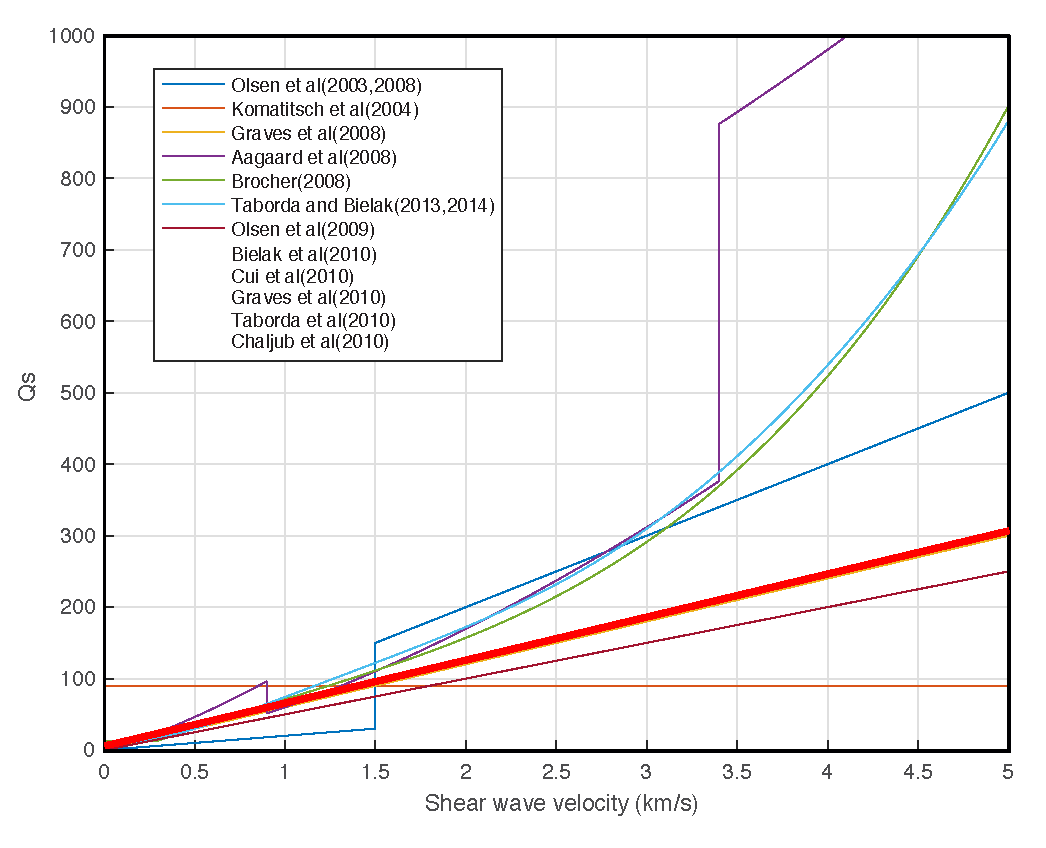
\includegraphics[width=400 px]{figures/pdf/Figure_q_models.pdf}
    \caption{Comparison of Qs rules introduced in table. ~\ref{tab:QsVstable}.}
    \label{fig:Figure_q_models}
\end{figure}

Our proposed relationship---although may not be the definitive one because of limited data used here--- is in agreement with the mean on these values. It is laid between $50Vs$ and $100Vs$ that is commonly used for this region (Lahabra paper, and some other references for 50Vs). Although there is a considerable variation on final dataset shown in Figure.~\ref{fig:results_conservative_with_regression}, the Q equation is not unique for all stations.  Q value is dependent on many other parameters which cause different spatial variation and the end goal is providing a community Q model where all parameters are involved. Variations in QP and QS may be related to porosity, temperature variations, heterogeneity, grain boundary sliding, and lithology. Also, some of the spatial variations in QP and QS appear to be terminated by local fault structure, where on one side of a fault the Q values may be significantly different than on the other \citep{hauksson2006attenuation}.  Moreover, heterogenous domain can cause scattering attention by a redistribution of energy as it is reflected, or converted by small-scale features. These effects may require frequency dependent Q studies \citep{frankel1991mechanisms}.  Also in the near surface sedimentary basin Q is very low \citep{abercrombie1997near}.\\

Therefore, variation of Q values for different stations in a heterogeneous medium are acceptable and predictable. It doubles the importance of the proposed approach where each stations are accurate for different different range of parameters. However, for the physics based ground motion simulation in low frequency, it is a common practice to consider Q only as a function of shear wave velocity. Application of proposed method on simplified, layered and heterogenous medium represents its strong potential and robust behavior towards estimating the most accurate parameters for each station.\\

As we discussed earlier, in several stations peak values of signals in observation (mostly PGV and PGA) are higher than without damping simulation. This can happen due to source parameters (e.g., seismic moment, slip function, ...). Therefore, on other option for better studying the parameters is including source parameters in the ANNs. This can increase the number of training data, however, will give opportunity of involving more stations in the final model.

 


